\subsection{Operation}\label{requirementspecification:operation}
\blindtext

%==================== Fully Dressed Use Cases ====================

\subsubsection{Use Case Diagram} \label{requirementspecification:usecasediagrams}

\blindtext
%For alle Use Cases hvor brugeren navigerer i undermenuer af hovedmenuen, gælder det, at brugeren har mulighed for at gå et skridt tilbage ved at trykke på en ”tilbage knap”. Fremover ved benævningen ”Systemet er operationelt” menes, at systemet er tilsluttet strømforsyning og at alt fungerer samt at systemet er tilsluttet ethernet.

\begin{figure}[H]
	\centering
	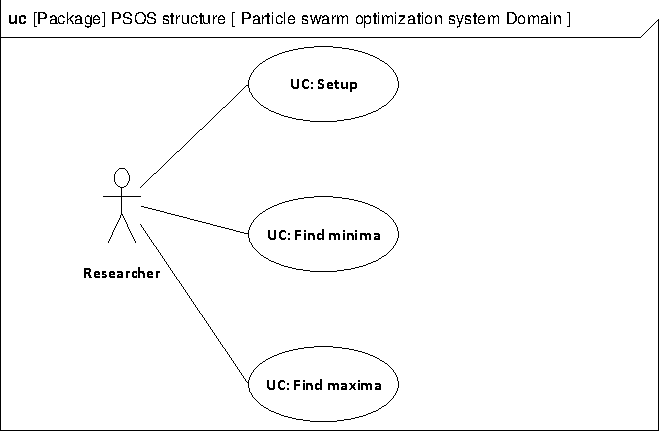
\includegraphics[width=0.8\linewidth]{diagram/uc_particle_swarm_optimization_system.pdf}
	\caption{Use Case Diagram of Particle Swarm Optimization}
	\label{fig:ucdiagram}
\end{figure}


%-------------------- UC1 --------------------
\begin{table}[h]
\begin{tabularx}{\textwidth}{| >{\raggedright\arraybackslash}p{3.3 cm} | >{\raggedright\arraybackslash}X |} \hline

\textbf{Name:} 						& UC1: Start\\ \hline
\textbf{Goal:}						&  \\ \hline
\textbf{Initering:}					&  \\ \hline
\textbf{Actor:} 					& User (primær) \\ \hline
\textbf{Reference:} 					& UC10: Monitorering, UC11: Regulering \\ \hline
\textbf{Number of simultaneous occurrences:} & Én \\ \hline
\textbf{Pre-condition:} 				& \\ \hline
\textbf{Result:}					&  \\ \hline
\textbf{Main scenario:}				& 

\begin{packed_enum}
\item allaa
\item allala
\item alllaa
	\begin{packed_item}\itemsep1pt \parskip0pt \parsep0pt
	\item {[}Ext 3.a : User does not press "Regulation".{]}
	\end{packed_item}
\item Systemet aktiverer UC11: Regulering.
\item UC1 afsluttes.
\end{packed_enum} \\ \hline
\textbf{extensions:}				&  
\textbf{{[}Ext 3.a :User selects only monitoring.{]}}
	\begin{packed_enum}\itemsep1pt \parskip0pt \parsep0pt
	\item The system continues at point. 5 in the main scenario.
	\end{packed_enum}
\\ \hline
\end{tabularx}
\caption{UC1: Start}
\label{tbl:uc1}
\end{table}
%-------------------- UC2 --------------------
\begin{table}[h]
	\begin{tabularx}{\textwidth}{| >{\raggedright\arraybackslash}p{3.3 cm} | >{\raggedright\arraybackslash}X |} \hline
		
		\textbf{Name:} 						& UC2: Find minima\\ \hline
		\textbf{Goal:}						& Find the minima of a function \\ \hline
		\textbf{Initering:}					& Researcher \\ \hline
		\textbf{Actor:} 					& Researcher (primary) \\ \hline
		\textbf{Reference:} 				& UC1: Setup \\ \hline
		\textbf{Number of simultaneous occurrences:} & One \\ \hline
		\textbf{Pre-condition:} 				& UC1 has been done \\ \hline
		\textbf{Result:}					& Found the minima of a function \\ \hline
		\textbf{Main scenario:}				& 
		
		\begin{packed_enum}
			\item allaa
			\item allala
			\item alllaa
			\begin{packed_item}\itemsep1pt \parskip0pt \parsep0pt
				\item {[}Ext 3.a : User does not press "Regulation".{]}
			\end{packed_item}
			\item Systemet aktiverer UC11: Regulering.
			\item UC1 afsluttes.
		\end{packed_enum} \\ \hline
		\textbf{extensions:}				&  
		\textbf{{[}Ext 3.a :User selects only monitoring.{]}}
		\begin{packed_enum}\itemsep1pt \parskip0pt \parsep0pt
			\item The system continues at point. 5 in the main scenario.
		\end{packed_enum}
		\\ \hline
	\end{tabularx}
\caption{UC2: Start}
\label{tbl:uc2}
\end{table}
%-------------------- UC3 --------------------
\begin{table}[h]
\begin{tabularx}{\textwidth}{| >{\raggedright\arraybackslash}p{3.3 cm} | >{\raggedright\arraybackslash}X |} \hline

\textbf{Navn:} 						& UC1: Start\\ \hline
\textbf{Mål:}						& At starte systemet helt eller delvist. \\ \hline
\textbf{Initering:}					& Bruger \\ \hline
\textbf{Aktører:} 					& Bruger (primær) \\ \hline
\textbf{Reference:} 					& UC10: Monitorering, UC11: Regulering \\ \hline
\textbf{Antal samtidige forekomster:} & Én \\ \hline
\textbf{Forudsætning:} 				& Systemet er stoppet helt, er operationelt og viser hovedmenuen.\\ \hline
\textbf{Resultat:}					& UC10: Monitorering og evt. UC11: Regulering er startet, systemet viser Hovedmenuen. \\ \hline
\textbf{Hovedscenarie:}				& 

\begin{packed_enum}
\item Bruger trykker på "Monitorering". 
\item System aktiverer UC10: Monitorering. 
\item Bruger trykker på "Regulering". 
	\begin{packed_item}\itemsep1pt \parskip0pt \parsep0pt
	\item {[}Ext 3.a : Bruger trykker ikke "Regulering".{]}
	\end{packed_item}
\item Systemet aktiverer UC11: Regulering.
\item UC1 afsluttes.
\end{packed_enum} \\ \hline
\textbf{Udvidelser:}				&  
\textbf{{[}Ext 3.a : Bruger vælger kun monitorering.{]}}
	\begin{packed_enum}\itemsep1pt \parskip0pt \parsep0pt
	\item Systemet fortsætter ved pkt. 5 i hovedscenariet.
	\end{packed_enum}
\\ \hline
\end{tabularx}
\caption{UC3: Start}
\label{tbl:uc3}
\end{table}

\subsubsection{Requirements}